\chapter{Úpravy desky plošného spoje proudového zdroje \emph{MoSeZ Rev. A}}

Při nové revizi desky (Rev. B) byl kladen důraz na zvýšení maximálního napájecího napětí z \SI{12}{\volt} na \SI{48}{\volt}, 
s možností pracovat již od \SI{12}{\volt}. 
Byly identifikovány a odstraněny některé problémy v původní verzi (Rev. A) proudového zdroje \textit{MoSeZ}. 
Rovněž byly rozšířeny funkce a věnována pozornost zmenšení velikosti desky plošného spoje.

Z pohledu součástkové základny byl značně zredukován počet druhů součástek. 
Operační zesilovače nejsou v nové revizi vůbec použity a druhy kondenzátorů a rezistorů byly výrazně sníženy. 
Zůstalo čtyřvrstvé \textit{DPS} (\textit{TOP} – \textit{IN1} – \textit{IN2} – \textit{BOT}), 
avšak vrstevní uspořádání bylo upraveno na \textit{SIGNÁL} – \textit{GND} – \textit{GND} – \textit{SIGNÁL} 
namísto původního \textit{SIGNÁL} – \SI{3,3}{\volt} – \textit{GND} – \textit{SIGNÁL}. 
Většina součástek byla přesunuta na \textit{TOP} stranu desky, 
zatímco na \textit{BOT} straně zůstaly pouze výkonové \textit{MOSFET} tranzistory a ochranné \textit{TVS} diody. 
Celkové rozměry desky byly zredukovány o přibližně \SI{21}{\percent}.

Další detailní úpravy jsou popsány v následujících podkapitolách, 
které odpovídají blokovému rozdělení v elektrickém schématu, viz obr. \ref{fig::block_diagram}.

\begin{figure}[htpb]
	\centering
	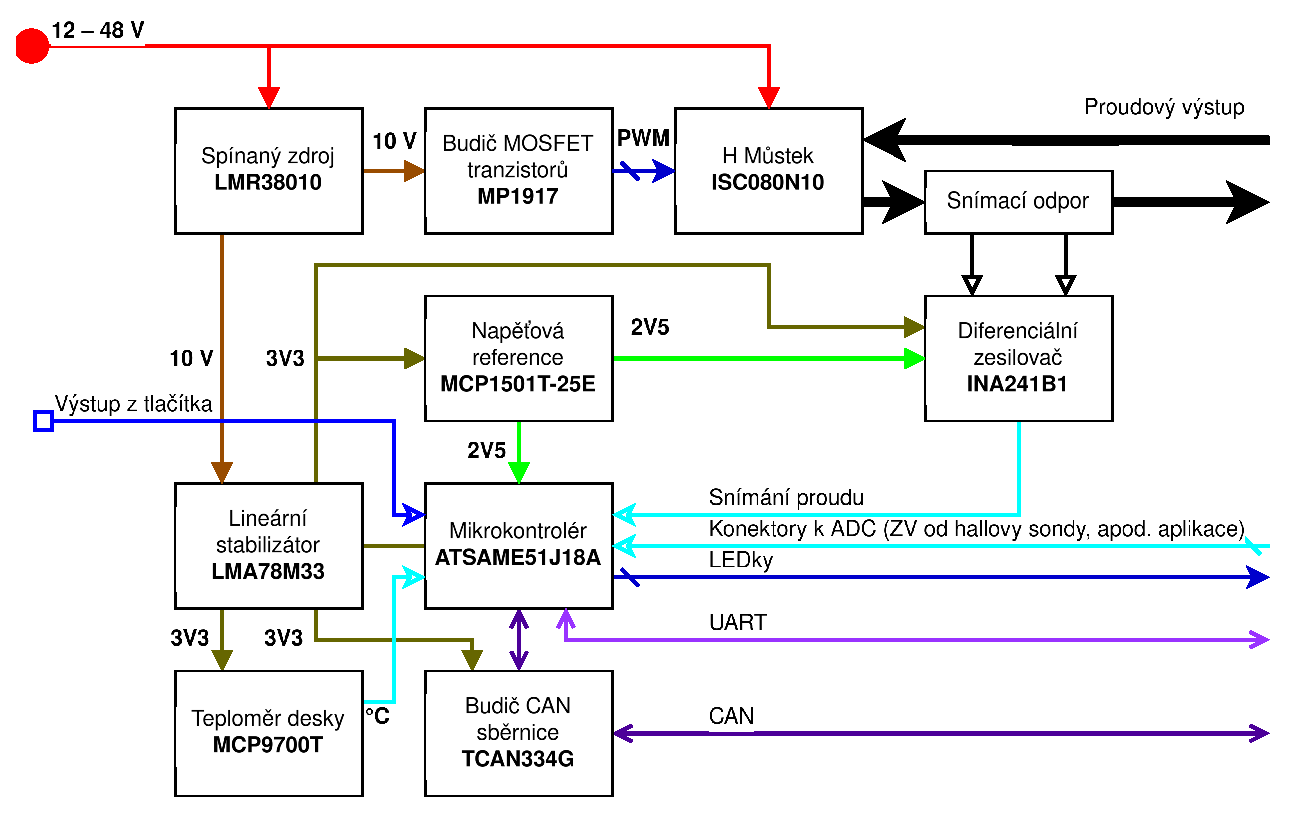
\includegraphics[width=0.9\textwidth]{kapitola2/figures/block_diagram.eps}
	\caption{Blokové schéma MoSeZ rev. B}
	\label{fig::block_diagram}
\end{figure}

\section{Vstupní obvody}

Vstupní obvody desky MoSeZ (rev. B) jsou navrženy tak,
aby zajistily spolehlivou ochranu a stabilní napájení.
Zvlnění vstupního napětí efektivně minimalizuje kombinace dvou elektrolytických kondenzátorů.
Pro ochranu proti přetížení jsou na vstupu dvě \textit{PTC} pojistky.
Jakmile proud překročí bezpečný limit, pojistky zvýší svůj odpor a odpojí napájení.
Proti přepólování je deska chráněna kombinací diody a \textit{PTC} pojistek,
zatímco varistor a \textit{TVS} dioda poskytují ochranu proti přepětí.
Měření vstupního napětí probíhá přes napěťový dělič,
který převádí maximální napětí na úroveň vhodnou pro analogově-digitální převodník mikrokontroléru.


\subsection{Vstupní elektrolytické kondenzátory}
\label{section::input_capacitors}
Minimální kapacitu vstupního kondenzátoru lze vypočítat podle jednoduchého vzorce:

\begin{equation}
	C_{\text{IN}} \geq \frac{I_{\text{LOAD}}}{f_{\text{SW}} \cdot \Delta U_{\text{ripple}}},
	\label{eq:min_capacity}
\end{equation}

kde:
\begin{itemize}
	\item $C_{\text{IN}}$ je minimální kapacita vstupního kondenzátoru ve \SI{}{\farad}
	\item $I_{\text{LOAD}}$ je proud zátěže v \SI{}{\ampere}
	\item $f_{\text{SW}}$ je spínací frekvence \SI{}{\hertz}
	\item $\Delta U_{\text{max\_zvlnění}}$ je maximální povolené zvlnění napětí \SI{}{\volt}
\end{itemize}

Maximální plánovaný výstupní proud zdroje \emph{MoSeZ} je $I_{\text{LOAD}} = \SI{8}{\ampere}$, 
ale pro rezervu ve výpočtech byl zvolen proud $I_{\text{LOAD}} = \SI{10}{\ampere}$.
Plánovaná spínací frekvence je $f_{\text{SW}} = \SI{100}{\kilo\hertz}$
a maximální přípustné zvlnění vstupního napětí bylo určeno na \SI{0,5}{\volt},
takže po dosazení do rovnice \eqref{eq:min_capacity} dostáváme:

\begin{equation}
	C_{\text{IN}} \geq \frac{10}{100 \cdot 10^3 \cdot 0,5}
\end{equation}

takže,

\begin{equation}
	C_{\text{IN}} \geq  240 \,\mu\mathrm{F}
\end{equation}

Zvolené zvlnění \SI{0,5}{\volt} zohledňuje napájecí napětí \SI{12}{\volt} a
potřebu dostatečné rezervy pro napájení pomocného spínaného zdroje \textit{LMR38010} (viz \nameref{section::smps_LMR38010}).
Tento pomocný zdroj zajišťuje výstupní napětí \SI{10}{\volt},
které je kritické pro napájení budičů \textit{MOSFET} tranzistorů \textit{MP1917}.
Napájecí napětí těchto budičů se totiž rovná spínacímu napětí na jejich výstupu (viz \cite{mp1917_ds}).
Pokud by spínací napětí MP1917 kleslo pod \SI{10}{\volt},
hrozilo by neúplné otevření hradel MOSFET tranzistorů,
což by mohlo vést k jejich přehřívání (viz \cite{ISC080N10NM6_ds}).
Vzhledem k tomu, že k významnému zvlnění dochází při vyšších výstupních proudech,
hrozí v takovém případě poškození tranzistorů vlivem tepelného průrazu.

Kvůli běžné toleranci kapacity elektrolytických kondenzátorů \SI{\pm 20}{\percent} jsem
pro filtraci napájení zvolil dvojici \SI{150}{\micro\farad} \textit{THT} kondenzátorů.
Použití \textit{THT} kondenzátorů v této kapacitní kategorii přináší finanční úsporu oproti povrchově montovaným (\textit{SMD}) kondenzátorům,
které byly použity v předchozí verzi desky \emph{MoSeZ} (rev. A).


\subsection{Nadproudová ochrana a ochrana proti přepolování}

Pro nadproudovou ochranu byly použity \textit{PTC} pojistky \textit{2920L150/60 od firmy Littelfuse}.
Oproti původnímu návrhu desky (\textit{MoSeZrev. A}) byl počet těchto pojistek snížen na dvě.
Každá z pojistek je dimenzována pro trvalý proud \SI{1,5}{\ampere},
což dohromady postačuje pro jištění trvalého proudu do \SI{3}{\ampere}.
Původní ochranná dioda byla nahrazena levnějším modelem \textit{BYG10D}.
Tato dioda spolu s \textit{PTC} pojistkami slouží jako ochrana proti přepólování.
V případě nechtěné záměny polarity napájecího napětí se dioda \textit{BYG10D} stane vodivou a zkratuje vstupní napětí.
Pokud proud z napájecího zdroje v takové situaci překročí \SI{3}{\ampere}, \textit{PTC} pojistky se zahřejí a obvod rozpojí.

V případě, kdy proud z napájecího zdroje nepřekročí prahový proud \textit{PTC} pojistek,
hrozí tepelný průraz diody \textit{BYG10D}.
To by ovšem znamenalo, že se dioda pravděpodobně stane trvale vodivou,
takže by došlo k vyřazení zdroje z provozu do doby její výměny.
Elektrolytické kondenzátory by však zůstaly ochráněny.

\section{Ochrana proti přepětí}

Pro ochranu proti přepětí na vstupu slouží kombinace varistoru a \textit{TVS} diody,
obě s pracovním napětím \SI{48}{\volt}.
Při návrhu je klíčové umístit tyto součástky co nejblíže vstupnímu konektoru.
Důležité je i jejich fyzické uspořádání od nejpomalejší po nejrychlejší,
tedy nejblíže ke vstupnímu konektoru varistor a za ním \textit{TVS} dioda.
Tím je zajištěno, že rychlá \textit{TVS} dioda omezí přepětí do doby, než se aktivuje varistor,
který následně převezme hlavní část svodového výkonu.
Varistory, jakožto pomalejší ochranné prvky, jsou schopny dlouhodobě svádět větší výkon než \textit{TVS} diody.
V případě opačného pořadí hrozí, že \textit{TVS} dioda bude muset odvést veškerý výkon,
protože na varistor, se nedostane žádné přepětí, což by mohlo vést ke zničení \textit{TVS} diody.


\subsection{Měření vstupního napětí}

Vstupní napětí je měřeno pomocí děliče napětí,
který je navržen tak, aby při \SI{48}{\volt} na vstupu dával na výstupu \SI{1,65}{\volt}.
Maximální napětí, které jsou schopny měřit AD převodníky použitého mikrokontroléru (viz \nameref{section::mcu_hw}),
je \SI{2,5}{\volt}, přičemž jsou tolerantní vůči napětí \SI{3,3}{\volt}.
To znamená, že jsou schopny měřit vstupní napětí až do \SI{106}{\volt}
a k poškození analogových vstupů MCU dojde až při napětí \SI{141}{\volt}.
Tato velká rezerva je zvolena z důvodu ochrany analogových vstupů mikrokontroléru,
a tím i jeho převodníku, před přepětím, nebo v případě, že by uživatel připojil příliš vysoké napětí.
Velikost vstupního napětí se nepoužívá pro regulaci a jeho znalost slouží pouze pro orientační měření.
Proto není kritická přesnost tohoto měření.


\section{Pomocný zdroj napětí \SI{10}{\volt}}
\label{section::smps_LMR38010}

V nové revizi \textit{DPS} zajišťuje \SI{10}{\volt} výstup pro budiče \textit{MOSFET} tranzistorů obvod \textit{LMR38010}.
Tento synchronní snižující měnič reguluje široký rozsah vstupního napětí
a minimalizuje potřebu externích ochranných součástek a
umožňuje nastavit spínací frekvenci v rozsahu \SI{200}{\kilo\hertz} až \SI{2.2}{\mega\hertz}.
Vestavěné ochrany zahrnují proudové omezení po jednotlivých cyklech,
ochranu proti zkratu a tepelnou ochranu při nadměrném vyzářeném výkonu.

\subsection{Výpočet velikosti odporů v napěťové zpětné vazbě}

Rovnice pro výpočet zpětnovazebního rezistoru z datasheetu viz \cite{mp1917_ds} říká, že

\begin{equation}
	R_{FBT} = \frac{U_{OUT} - U_{REF}}{U_{REF}} \cdot R_{FBB},
	\label{eq:lmr_fb}
\end{equation}

kde

\begin{enumerate}
	\item \(R_{FBT} \) : Odpor horního rezistoru (mezi \(U_{OUT} \) a \textit{FB} pinem), měl by vyjít v rozmezí mezi \SI{10}{\kilo\ohm} až \SI{100}{\kilo\ohm}.
	\item \(U_{OUT} \) : Požadované výstupní napětí stabilizátoru.
	\item \(U_{REF} \) : Referenční napětí, \SI{1}{\volt} pro \textit{LMR38010}.
	\item \(R_{FBB} \) : Odpor dolního rezistoru (mezi FB pinem a zemí).
\end{enumerate}

dosazením $ \quad U_{OUT} = \SI{10}{\volt}$ a $R_{FBB} = \SI{10}{\kilo\ohm}$ dostávám:

\begin{equation}
	R_{FBT} = 9 \cdot 10 \cdot 10^3 = \SI{90}{\kilo\ohm}
\end{equation}

Nicméně pro unifikaci pasivních součástek byl zvolen $ \quad R_{FBT} = \SI{100}{\kilo\ohm}$ a $R_{FBB} = \SI{10}{\kilo\ohm}$,
takže upravení rovnice \eqref{eq:lmr_fb} dostávám výstupní napětí pro tuto kombinaci, asice:

\begin{equation}
	U_{OUT} = U_{REF} \cdot \left(\frac{R_{FBT}}{R_{FBB}} + 1 \right) = 1 \cdot \left(\frac{100}{10} + 1 \right) = \SI{11}{\volt}.
	\label{eq:lmr_vout_real}
\end{equation}


Těmito \SI{11}{\volt} jsou napájeny budiče \textit{MP1917},
což znamená, že se zároveň jedná o napětí,
kterými budou budiče spínat gaty \textit{MOSFET} transistorů, viz \cite{mp1917_ds}.
Napětí \SI{11}{\volt} je dle datasheetu tranzistorů \textit{ISC080N10} přípustná velikost spínacího napětí gatů,
viz \cite{ISC080N10NM6_ds}.


\subsection{Výpočet velikosti odboru programujícího spínací kmitočet}


Rovnice pro výpočet odporu RT z datasheetu \cite{mp1917_ds} říká, že

\begin{equation}
	R_{T} = 30970 \cdot f_{SW}^{-1,027},
	\label{eq:lmr_rt}
\end{equation}

kde

\begin{enumerate}
	\item $R_{T}$ : Odpor mezi pinem textit{RT/SYNC} a zemí, udávaný v\SI{}{\kilo\ohm}.
	\item $f_{SW}$ : Spínací frekvence, udávaná v \SI{}{\kilo\hertz}.
\end{enumerate}

Pro unifikaci pasivních součástek byl zvolen R\_{T} = \SI{50}{\kilo\ohm},
respektive paralelní kombinace dvou \SI{100}{\kilo\ohm} odborů použitých v napěťové zpětné vazbě \textit{LMR38010}.
Upravením rovnice \eqref{eq:lmr_rt} dostávám skutečnou spínací frekvenci pro tuto hodnotu terminačního odporu, a sice:

\begin{equation}
	f_{SW} = \left(\frac{R_T}{30970} \right)^{-\frac{1}{1,027}} =
	\left(\frac{50}{30970} \right)^{-\frac{1}{1,027}} \approx \SI{628}{\kilo\hertz}.
	\label{eq:lmr_fsw_real}
\end{equation}

Vyšší spínací frekvence umožňují použití menších induktorů a kondenzátorů ve výstupním LC filtru,
což vede k úspoře místa a potenciálně lepší dynamické odezvě měniče.
Nicméně s rostoucí frekvencí se zvyšují ztráty způsobené parazitními kapacitami
a svody v pasivních součástkách i na plošném spoji, což může negativně ovlivnit účinnost,
zejména při nízkých výstupních výkonech.
Při velmi malých zátěžových proudech a vysokých spínacích frekvencích mohou tyto parazitní ztráty tvořit významnou část celkového výkonu,
a proto bývá výhodnější zvolit nižší spínací frekvenci, kde jsou tyto ztráty menší.
Optimální volba spínací frekvence tak závisí na kompromisu mezi velikostí pasivních součástek,
účinností a požadavky na elektromagnetickou kompatibilitu (EMI), viz \cite{buck_switching_freq_affection}


\subsection{Výpočet velikosti výstupního dolnopropustého LC filtru}

LC filtr je nezbytnou součástí každého spínaného zdroje, zejména pokud má na výstupu stejnosměrné napětí.
Pro správný výběr induktoru jsou klíčové hodnota indukčnosti a saturační proud.
Indukčnost se obvykle volí tak, aby zvlnění výstupního proudu bylo mezi \SI{20}{\percent} a \SI{40}{\percent}.

Pro výpočet minimální indukčnosti platí vztah:

\begin{equation} L \geq \frac{(U_{IN} - U_{OUT})}{f_{SW} \cdot K \cdot I_{OUT(MAX)}} \cdot \frac{U_{OUT}}{U_{IN}}. \label{eq:lmr_inductance} \end{equation}

Saturační proud induktoru by měl být alespoň tak velký jako maximální očekávaný výstupní proud, aby se zabránilo jeho nasycení.
Pro spínací frekvence nad \SI{1}{\mega\hertz} se doporučují induktory s feritovým jádrem kvůli nižším ztrátám.

Maximální výstupní proud $ I_{OUT(MAX)} $ byl zvolen \SI{0,5}{\ampere} pro zajištění dostatečné výkonové rezervy.
I přes špičkové odběry budičů se očekává, že střední hodnota výstupního proudu bude výrazně nižší.
Minimální napájecí napětí bylo stanoveno na $U_{IN} = \SI{12}{\volt}$
a požadované výstupní napětí $U_{OUT} = \SI{11}{\volt}$, viz rovnice \eqref{eq:lmr_vout_real}.
Koeficient zvlnění proudu byl zvolen $K = 0,2$ (tj. \SI{20}{\percent}) a
spínací frekvence $f_{SW} = \SI{628}{\kilo\hertz}$, viz rovnice \eqref{eq:lmr_fsw_real}.

Dosazením do rovnice \eqref{eq:lmr_inductance} dostáváme:

\begin{equation} L \geq \frac{(12 - 11)}{628 \cdot 10^3 \cdot 0,2 \cdot 0,5} \cdot \frac{11}{12} \approx \SI{29,3}{\micro\henry}. \end{equation}

Dle doporučení v datasheetu \cite{mp1917_ds} byla zvolena nejbližší vyšší vyráběná hodnota, tedy $L = \SI{33}{\micro\henry}$.

Minimální kapacita $C_{OUT}$ byla určena podle vztahu, který neuvažuje statické zvlnění,
ale zaměřuje se na schopnost zdroje reagovat na skokové změny výstupního proudu.
To je klíčové, protože zdroj bude primárně napájet budiče \textit{MOSFET} tranzistorů,
kde dochází k rychlým změnám odběru.

\begin{equation}
	C_{OUT} \geq \frac{\Delta I_{OUT}^2 \cdot L}{2 \cdot U_{OUT} \cdot U_{\text{zvlnění}}}
	\label{eq:cout_min_cap_smps}
\end{equation}

kde:

\begin{itemize}
	\item $C_{OUT}$ : Minimální kapacita výstupního kondenzátoru pro omezení překmitu napětí.
	\item $\Delta I_{OUT}$ : Maximální změna výstupního proudu v aplikaci.
	\item $L$ : Indukčnost cívky.
	\item $U_{OUT}$ : Výstupní napětí.
	\item $U_{\text{zvlnění}}$ : Maximální povolená změna výstupního napětí vlivem proudového skoku.
\end{itemize}

Pokud dosadíme následující parametry:

$\Delta I_{OUT} = \SI{1}{\ampere}, \quad
	L = \SI{33}{\micro\henry}, \quad
	U_{OUT} = \SI{11}{\volt}, \quad
	U_{\text{zvlnění}} = \SI{50}{\milli\volt}$
do rovnice \eqref{eq:cout_min_cap_smps}, dostaneme:

\begin{equation}
	C_{OUT} \geq \frac{1^2 \cdot 33 \cdot 10^{-6}}{2 \cdot 11 \cdot 50 \cdot 10^{-3}} \approx \SI{30}{\micro\farad}.
\end{equation}

Na filtraci jsou použity keramické kondenzátory s dielektrikem \textit{X7R} dimenzované na napětí \SI{25}{\volt}.
Keramika \textit{X7R} má následující vlastnosti:

\begin{itemize}
	\item \textbf{Snížení kapacity při DC napětí} – při $\frac{1}{2}$ nominálního napětí a
	      pokojové teplotě je kapacita až o \SI{30}{\percent} nižší než nominální hodnota.
	\item \textbf{Teplotní drift} – změna kapacity až $\pm15\%$ v rozsahu \SI{-50}{\degreeCelsius} až \SI{+125}{\degreeCelsius}.
	\item \textbf{Stárnutí materiálu} – kapacita klesá o jednotky procent v čase.
\end{itemize}

Vzhledem k těmto faktorům a snaze unifikovat součástky na desce \emph{MoSeZ} byla použita kombinace:

\begin{itemize}
	\item $3 \cdot \SI{22}{\micro\farad}$ keramické kondenzátory \textit{X7R}.
	\item $1 \cdot \SI{100}{\nano\farad}$ keramický kondenzátor umístěný co nejblíže k cívce pro redukci vysokofrekvenčního rušení.
\end{itemize}

Tato kombinace zajišťuje \textbf{dostatečnou rezervu kapacity}, \textbf{nižší ESR} a \textbf{lepší potlačení rušení}.

\subsection{Vstupní filtrační kondenzátory}

Na vstupu je pouze paralelní kombinace dvou \SI{22}{\nano\farad} kondenzátorů pro filtraci vysokofrekvenčního rušení.
Další kondenzátory s vyšší kapacitou byly z návrhu vyřazeny.
Důvodem je umístění obvodu \textit{LMR38010} v těsné blízkosti velkých vstupních filtračních kondenzátorů
(viz \nameref{section::input_capacitors}).
Vzhledem k této skutečnosti se ukázalo použití lokálních filtračních kondenzátorů s větší kapacitou jako zbytečné.
Toto řešení přineslo značnou prostorovou úsporu na DPS,
což bylo velmi výhodné, protože v oblasti usazení obvodu \textit{LMR38010} byl prostor velmi omezený.

\section{Pomocný zdroj napětí \SI{3,3}{\volt}}
\label{sec::linear_lm78}

Napětí \SI{3,3}{\volt} pro mikroprocesor a 
ostatní obvody jako \textit{TCAN334G}, \textit{INA241B1},
či \textit{MCP1501T}  obstarává obvod \textit{LMA78M33}.
Jedná se o lineární stabilizátor napájený \SI{10}{\volt} výstupu z \textit{LMR38010}, viz \nameref{section::smps_LMR38010}.
Filtrační kondenzátory byly zvoleny dle jasného doporučení v datasheetu bez jakýchkoliv kalkulací,
viz \cite{LM78M_ds}.
Samotý obvod je tak jednoduchý a obecně známý, že nemá cenu o něm cokoliv více psát.

V původní verzi zdroje byly pro snižování vstupního napětí použity dva snižující měniče v integrovaném obvodu \textit{MP2344}.
Tyto obvody poskytovaly napětí \SI{10}{\volt} pro napájení budičů \textit{MOSFET} tranzistorů a \SI{3,3}{\volt} pro napájení mikroprocesoru.
V důsledku náhodných přepětí na výstupu těchto obvodů docházelo k poškození mikroprocesorů.
Záměnou řešení s \textit{MP2344} se podařilo problém odstranit,i když to nemusela být vina obvodů jako takových,
ale například špatného návrhu snižujících měničů. 
Nové řešení s \textit{LM78M33} je v každém případě mnohem jednodušší a levnější.

\section{Mikrokontrolér}
\label{section::mcu_hw}

V mikrokontroléru bude implementovaný regulátor a bude obstarávat veškerou komunikaci,
včetně zpracovávání vstupů z tlačítka a rozsvicování indikačních \textit{LED}.
Nová revize využívá stejný typ mikrokontroléru, asice \textit{ATSAME51J20A}.
V původním návrhu desky byl jako zdroj kmitočtu pro mikroprocesor použit \SI{32}{\kilo\hertz} krystalový rezonátor.
Tento rezonátor způsoboval nespolehlivé spouštění při inicializaci procesoru.
V nové verzi desky byl použit \SI{20}{\mega\hertz} rezonátor, 
který byl ověřen v jiných projektech s \textit{MCU} od \textit{Microchip}.
Došlo také k opravě záměny pinů programovacího konektoru \textit{SWDIO} a \textit{SWDCLK},
což byla chyba v původním návrhu desky \textit{MoSeZ}, která vedla k výrobě specialního programovacího kabelu.

Každý digitální napájecí vstupní pin \textit{VDDIO} je odfiltrován keramickým kondenzátorem s kapacitou \SI{100}{\nano\farad}.
Ke spínanému zdroji integrovaného v mikrokontroléru je připojena indukčnost o velikosti \SI{10}{\micro\henry},
která filtruje výstupní proud a za ni je pro filtrování vzniklého napětí \textit{VDDCORE} připojena kombinace \SI{22}{\micro\farad} a \SI{100}{\nano\farad} kondenzátorů.
Analogové napětí \textit{VDDANA} se tvoří z napětí \textit{VDDIO} přes LC filtr tvořený dvěma kondenzátory a feritovou perličkou zapojenými do $\pi$ článku.
Kondenzátory mají kapacitu \SI{22}{\micro\farad} a feritová perlička o impedanci \SI{330}{\ohm} na frekvenci \SI{100}{\mega\hertz}.
Součástky byly vybrány a zapojeny dle doporučení v datasheetu, viz \cite{ATSAME51J20A_ds}.


\section{Proudový výstup}

Řízení elektromagnetických aktuátorů vyžaduje spolehlivý a výkonný proudový výstup, 
který je schopen generovat obousměrné stejnosměrné (DC) a střídavé (AC) signály s požadovanými parametry. 
Z tohoto důvodu byla v rámci proudových zdrojů \textit{MoSeZ} navržena výstupní část založená na topologii \textit{H-můstku}, 
která umožňuje obousměrný tok proudu a generování dynamicky tvarovaných průběhů.
Klíčovými aspekty návrhu výstupního obvodu jsou vhodná volba výkonových tranzistorů, 
účinné řízení spínacích prvků a tepelný management. 
V následujících podsekcích jsou rozebrány konstrukční i výpočetní aspekty této části obvodu.



\subsection{H-můstek}

Tranzistory \textit{MOSFET} původní revize desky \textit{MoSeZ} by nemohly pracovat na napětí \SI{48}{\volt}, 
proto bylo nutné zvolit nové tranzistory s parametrem \(U_{DS\_MAX} > 2 \cdot \SI{48}{\volt}\). 
Výběr padl na \textit{Infineon ISC080N10}, u kterého bylo nutné ověřit, 
že může být dlouhodobě zatěžován proudem \SI{8}{\ampere} bez rizika tepelného průrazu. 
Maximální proud do zátěže bude uvažován jako \SI{10}{\ampere}, což zajistí určitou výkonovou rezervu.

Pro výpočet celkových ztrát na \textit{MOSFET} tranzistoru se dle \cite{mosfet_losses} se používá následující vztah:

\begin{equation}
    P_{LOSS} = P_{J} + P_{SW} + P_{G}
\end{equation}

kde:

\begin{itemize}
    \item \(P_{LOSS}\): Celkové ztráty na \textit{MOSFET} tranzistoru.
    \item \(P_{J}\): Ztráty způsobené odporem kanálu \textit{MOSFET} tranzistoru (vodivostní ztráty).
    \item \(P_{SW}\): Ztráty vznikající při spínání a rozepínání tranzistoru (spínací ztráty).
    \item \(P_{G}\): Ztráty způsobené kapacitou gate tranzistoru (ztráty hradlem).
\end{itemize}

Vodivostní ztráty se vypočítají jako:

\begin{equation}
    P_{J} = I_{D}^{2} \cdot R_{DS\_ON}
    \label{eq:joullossesfet}
\end{equation}

kde ze zadání a datasheetu \cite{ISC080N10NM6_ds}:

\begin{itemize}
    \item \(I_D\): Proud protékající tranzistorem (Drain current) – \SI{10}{\ampere}.
    \item \(R_{DS\_ON}\): Odpor kanálu tranzistoru v sepnutém stavu (Drain-source resistance on-state) – \SI{8.5e-3}{\ohm}.
\end{itemize}

Dosazením těchto hodnot do rovnice \eqref{eq:joullossesfet} dostaneme:

\begin{equation}
    P_{J} = 10^2 \cdot 8.5 \cdot 10^{-3} = \SI{0,85}{\watt}
\end{equation}

Spínací ztráty se vypočítají jako:

\begin{equation}
    P_{SW} = 0,5 \cdot U_{CC} \cdot I_{D} \cdot (t_{r} + t_{f}) \cdot f_{SW}
    \label{eq:switchingFETlosses}
\end{equation}

kde dle zadání a datasheetu \cite{ISC080N10NM6_ds}:

\begin{itemize}
    \item \(U_{CC}\): Napájecí napětí – \SI{48}{\volt}.
    \item \(t_{r}\): Náběžná doba spínání – \SI{2,9e-9}{\second}.
    \item \(t_{f}\): Sestupná doba spínání – \SI{2,6e-9}{\second}.
    \item \(f_{SW}\): Spínací frekvence – \SI{100}{\kilo\hertz}.
\end{itemize}

Dosadíme tyto hodnoty do rovnice \eqref{eq:switchingFETlosses}:

\begin{equation}
    P_{SW} = 0,5 \cdot 48 \cdot 10 \cdot 2,9 \cdot 10^{-9} + 2,6 \cdot 10^{-9} \cdot 100 \cdot 10^{3} = \SI{0,1392}{\watt}
\end{equation}

Ztráty hradlem se vypočítají jako:

\begin{equation}
    P_{G} = Q_{G} \cdot U_{CC} \cdot f_{SW}
    \label{eq:FETleakgatelosses}
\end{equation}

kde dle předchozích výpočtů a datasheetu \cite{ISC080N10NM6_ds}:

\begin{itemize}
    \item \(Q_{G}\): Celkový náboj hradla (gate charge total) – \SI{2,38e-8}{\coulomb}.
\end{itemize}

Pro výše uvedené parametry, po dosazení do rovnice \eqref{eq:FETleakgatelosses} dostáváme:

\begin{equation}
    P_{G} = 2,38 \cdot 10^{-8} \cdot 48 \cdot 100 \cdot 10^{3} = \SI{0,1142}{\watt}
\end{equation}

Celkové ztráty se vypočítají jako součet všech ztrát:

\begin{equation}
    P_{LOSS} = P_{J} + P_{SW} + P_{G} = 0,85 + 0,1392 + 0,1142 = \SI{1,1034}{\watt}
\end{equation}

Maximální přípustné ztráty tranzistoru při chlazení footprintem DPS lze určit jako:

\begin{equation}
    P_{Z\_MAX} = \frac{T_{J\_MAX} - T_{\text{SURR}}}{R_{\text{thJA}}}
\end{equation}

kde dle datasheetu \cite{ISC080N10NM6_ds}:

\begin{itemize}
    \item \(T_{J\_MAX}\): Maximální přípustná teplota přechodu tranzistoru – \SI{175}{\celsius}.
    \item \(T_{\text{SURR}}\): Okolní teplota – \SI{50}{\celsius} (určeno jako teplota okolí s velkou rezervou).
    \item \(R_{\text{thJA}}\): Tepelný odpor tranzistor-okolí – \SI{75}{\kelvin\per\watt}. 
	Dle datasheetu \cite{ISC080N10NM6_ds} je \SI{50}{\kelvin\per\watt} pro \SI{6}{\centi\meter^2}. 
	Ačkoliv plánuji ještě větší chladící plochu, pro jistotu jsem přidal rezervu.
\end{itemize}

Po dosazení:

\begin{equation}
    P_{Z\_MAX} = \frac{175 - 50}{75} = \SI{1,6667}{\watt} > P_{LOSS} % Opraveno na >
\end{equation}

Takže tranzistor by neměl mít s provozem \SI{8}{\ampere} sebemenší problém. 
Teplota přechodu se při těchto provozních parametrech dá spočítat jako:

\begin{equation}
    T_{J} = T_{\text{SURR}} + P_{LOSS} \cdot R_{\text{thJA}}
\end{equation}

Po dosazení hodnot známých z předchozích výpočtů dostaneme:

\begin{equation}
    T_{J} = \SI{50}{\celsius} + \SI{1,1034}{\watt} \cdot \SI{75}{\kelvin\per\watt} = \SI{132,758}{\celsius} % Opraveno na 132,758
\end{equation}

Vypočtená teplota přechodu \SI{132,758}{\celsius} je mnohem nižší než maximální výrobcem přípustná teplota \SI{175}{\celsius}, 
takže tranzistor by měl být schopen pracovat bez rizika tepelného průrazu s relativně slušnou teplotní rezervou.
Proudový výstup je chráněn proti náhodným přepětím dvěma \textit{TVS} diododami s pracovním napětím \SI{48}{\volt},
viz \pref{priloha:schema_CurrentOutput}.


\subsection{Budiče tranzistorů}

Jsou využity dva budiče \textit{MOSFET} tranzistorů \textit{MP1917}.
Každý je řízen dvěma \textit{PWM} signály, z nichž jeden je pro řízení \textit{low-side} tranzistoru a
druhý pro řízení \textit{high-side} tranzistoru.
\textit{High-side} tranzistor je označován jako plovoucí, protože jeho \textit{Source} elektroda není přímo spojen se zemí,
ale je připojen k zátěži a \textit{low-side} tranzistoru.
Proto je výhodnější použít speciálně navržené budiče.
Pro otevření \textit{low-side} tranzistoru by stačil i napěťově zesílený signál z mikrokontroléru, což neplatí pro \textit{high-side} tranzistor.
Podmínka pro otevření libovolného \textit{MOSFET} tranzistoru je:

\begin{equation}
	U_{G} > U_{T} + U_{S}
\end{equation}

kde:

\begin{itemize}
	\item \(U_{G}\): Napětí na gate elektrodě tranzistoru.
	\item \(U_{T}\): Prahové napětí \textit{MOSFET} tranzistoru, tj. napětí při kterém se začíná otevírat (konstanta součástky).
	\item \(U_{S}\): Napětí na source elektrodě transistoru.
\end{itemize}

Pro \textit{high-side} tranzistor H-můstku platí:

\begin{equation}
	U_{GSH} > U_{T} + U_{LOAD} + U_{LS\_MOSFET}
\end{equation}

kde:

\begin{itemize}
	\item \(U_{LOAD}\): Napětí na zátěži.
	\item \(U_{LS\_MOSFET}\): Napětí na \textit{low-side} tranzistoru.
\end{itemize}

Pro plné otevření tranzistoru je nutné napětí výrazně vyšší než prahové napětí \(U_{T}\).
Tranzistory \textit{ISC080N10} jsou podle datasheetu plně otevřeny při \(U_{GS} = \SI{10}{\volt}\),
přičemž \(U_{GSMAX} = \SI{20}{\volt}\) (viz \cite{ISC080N10NM6_ds}).
Pro plné otevření tedy platí:

\begin{equation}
	U_{GSH} \ge \SI{10}{\volt} + U_{LOAD} + U_{LS\_MOSFET} < \SI{20}{\volt}
	\label{eq:mosfet_hs_opening_floatin}
\end{equation}

Napětí na zátěži \(U_{LOAD}\) a napětí na \textit{low-side} tranzistoru \(U_{LS\_MOSFET}\) jsou závislé na velikosti proudu protékajícího zátěží.
Z rovnice \eqref{eq:mosfet_hs_opening_floatin} vyplývá,
že i napětí potřebné pro otevření \textit{high-side} tranzistoru \(U_{GSH}\) se mění (plave), odtud název „plovoucí“ tranzistor.
Jednou z nejčastěji používaných metod,
jak splnit nerovnici \eqref{eq:mosfet_hs_opening_floatin},
je použití \textit{bootstrap} kondenzátoru a \textit{bootstrap} diody.

Bootstrap kondenzátor slouží jako zdroj napětí pro \textit{high-side} \textit{CMOS} budič,
který je v tomto případě integrován v \textit{MP1917}.
Kondenzátor musí být jednou elektrodou připojen přes \textit{bootstrap} diodu k napájecímu napětí budiče a
druhou elektrodou k potenciálu sourcu \textit{MOSFET} tranzistoru,
respektive k potenciálu zátěže.
Na obrázku \ref{fig::bootstrap_explained_LS_ON} je vidět,
že při sepnutí \textit{low-side} tranzistoru protéká zátěží proud \(I_{LOAD}\) a na zátěži vzniká úbytek \(U_{LOAD}\).
Zároveň je nabíjen \textit{bootstrap} kondenzátor napájecím napětím budiče,
v \oref{fig::bootstrap_explained_LS_ON} jako \(U_{DD} = \SI{10}{\volt}\),
přes \textit{bootstrap} diodu na napětí:

\begin{equation}
	U_{BSC} = \SI{10}{\volt} - U_{D} -  U_{LS} \approx \SI{10}{\volt}
	\label{eq:bootstrap_voltage_LSON}
\end{equation}

\begin{figure}[htpb]
	\centering
	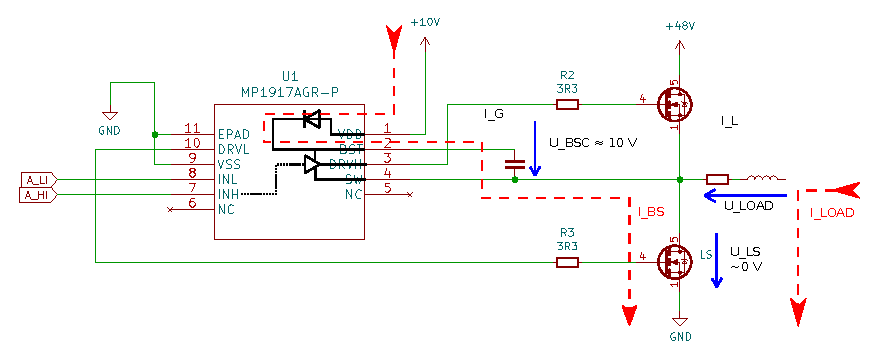
\includegraphics[width=0.9\textwidth]{kapitola2/figures/bootstrap_explained_LS_ON.eps}
	\caption{Nabíjení \textit{bootstrap} kondenzátoru přes sepnutý \textit{low-side} tranzistor na napájecí napětí budiče (\SI{10}{\volt}).}
	\label{fig::bootstrap_explained_LS_ON}
\end{figure}

Při rozepnutí tranzistoru \textit{LS} přestává být spodní elektroda kondenzátoru uzemněna a dostává se na potenciál zátěže, takže:

\begin{equation}
	U_{BSC} = \SI{10}{\volt} +  U_{LOAD}
	\label{eq:bootstrap_voltage_LSOFF} % Změněno na LSOFF pro konzistenci
\end{equation}

V tomto momentě zabraňuje vybíjení kondenzátoru \textit{bootstrap} dioda a
na \textit{bootstrap} kondenzátoru se udržuje napětí \(U_{DD} + U_{LOAD}\) vůči zemi.
Při sepnutí \textit{high-side} tranzistoru se toto napětí připojí na gate \textit{MOSFET} tranzistoru,
v \oref{fig::bootstrap_explained_LS_ON} označené jako \(U_{G}\),
a do gatu tranzistoru začne protékat vyrovnávací proud \(I_{G}\),
dokud se kapacita \(C_{G}\) nenabije na napětí \(U_{G}\). Tím je zajištěno, že

\begin{equation}
	U_{GS} = U_{BSC} \approx \SI{10}{\volt}
	\label{eq:bootstrap_voltage_lsoff} % Změněno na lsoff pro konzistenci
\end{equation}

a je dosaženo spínání \textit{high-side} tranzistoru.
Z popsaného principu je jasné, že \textit{high-side} tranzistor nemůže být spínán se střídou \SI{100}{\percent},
protože \textit{bootstrap} kondenzátor musí být nabíjen spínáním \textit{low-side} tranzistoru, viz \oref{fig::bootstrap_explained_LS_ON}.
V současnosti jsou \textit{bootstrap} diody běžně integrovány v budičích,
takže při návrhu stačí zvolit vhodný \textit{bootstrap} kondenzátor.

\begin{figure}[htpb]
	\centering
	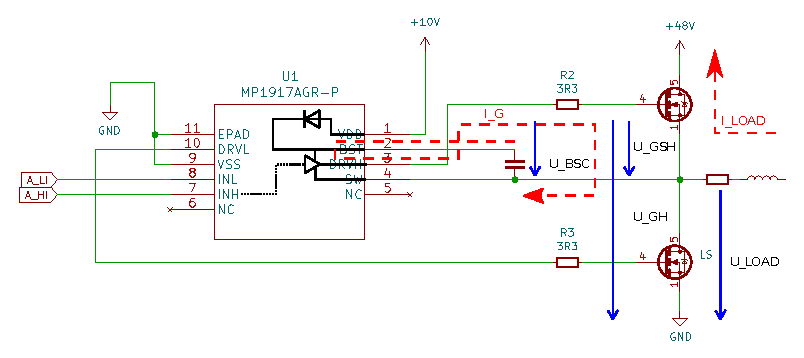
\includegraphics[width=0.9\textwidth]{kapitola2/figures/bootstrap_explained_LS_OFF.eps}
	\caption{Sepnutí \textit{high-side} tranzistoru pomocí součtu napětí na \textit{bootstrap} kondenzátoru a napětí zátěže. Směr proudu zátěží \(I_{LOAD}\) zachován z \oref{eq:bootstrap_voltage_LSON}}
	\label{fig::bootstrap_explained_LS_OFF}
\end{figure}

Tranzistory \textit{Infineon ISC080N10} mají téměř dvojnásobnou kapacitu hradla oproti původním Infineon \textit{BSZ0703L} (\emph{MoSeZ} revize A).
Proto bylo nutné přepočítat hodnoty \textit{bootstrap} kondenzátorů pro budiče \textit{MP1917}.
Výpočet minimální kapacity \textit{bootstrap} kondenzátoru \(C_{\textit{bootstrap}}\) se provádí pomocí provnic \eqref{eq:cboot_min_cap} až \eqref{eq:delta_uhs}
převzatých z \cite{bootstrap_moudra}:

\begin{equation}
	C_{\textit{bootstrap}} \geq \frac{Q_{total}}{\Delta U_{BSTQ}}
	\label{eq:cboot_min_cap}
\end{equation}

kde:

\begin{itemize}
	\item \(C_{\textit{bootstrap}}\): Minimální požadovaná kapacita \textit{bootstrap} kondenzátoru.
	\item \(Q_{total}\): Celkový náboj potřebný pro nabití a udržení hradla \textit{MOSFET} tranzistoru v otevřeném stavu.
	\item \(\Delta U_{BSTQ}\): Maximální přípustný pokles napětí na \textit{bootstrap} kondenzátoru během spínacího cyklu.
\end{itemize}

Celkový náboj \(Q_{total}\) se vypočítá podle vztahu:

\begin{equation}
	Q_{total} = Q_G + I_{DDQ} \cdot \frac{D_{max}}{f_{sw}} + I_{BSTQ} \cdot \frac{1-D_{max}}{f_{sw}}
	\label{eq:qtotal}
\end{equation}

kde:

\begin{itemize}
	\item \(Q_G\): Celkový náboj hradla vybraného \textit{MOSFET} tranzistoru.
	\item \(I_{DDQ}\): Klidový (svodový) proud \textit{\textit{high-side}} budiče.
	\item \(I_{BSTQ}\): Klidový (svodový) proud \textit{bootstrap} obvodu budiče.
	\item \(D_{max}\): Maximální střída \textit{PWM} signálu,
	      v desetiném vyjádření (např. 0.985 pro \SI{98.5}{\percent}).
	\item \(f_{sw}\): Spínací frekvence \textit{PWM} signálu.
\end{itemize}


Dosazením konkrétních hodnot z datasheetu \cite{mp1917_ds}:
\(Q_G = \SI{19}{\nano\coulomb}\),
\(I_{DDQ} = \SI{150}{\micro\ampere}\),
\(I_{BSTQ} = \SI{90}{\micro\ampere}\),
\(D_{max} = 0.985\), \(f_{sw} = \SI{100}{\kilo\hertz}\),
lze vypočíst hodnotu celkového \(Q_{total}\) dle rovnice \eqref{eq:qtotal} jako:


takže

\begin{equation}
	Q_{total} = 19 \cdot 10^{-9} + 150 \cdot 10^{-6} \cdot \frac{0,985}{100 \cdot 10^{3}} + 
	90 \cdot 10^{-6} \cdot \frac{1-0,985}{100 \cdot 10^{3}} \approx \SI{20,48}{\nano\coulomb},
\end{equation}

Maximální přípustný pokles napětí na \textit{bootstrap} kondenzátoru \(\Delta V_{BSTQ}\) se určí z rovnice:

\begin{equation}
	\Delta V_{BSTQ} = U_{DD} - U_{DH} - U_{UPFT} = U_{DD} - U_{DH} - U_{UPRT} - U_{HT}
	\label{eq:delta_uhs}
\end{equation}

kde:

\begin{itemize}
	\item \(U_{DD}\): Napájecí napětí budiče hradla \textit{IC}.
	\item \(U_{DH}\): Úbytek napětí na \textit{bootstrap} diodě.
	\item \(U_{UPFT}\): Prahová hodnota podpěťové ochrany budiče při poklesu napětí na napájecím pinu.
	\item \(U_{UPRT}\): Prahová hodnota podpěťové ochrany budiče při náběhu napětí na napájecím pinu.
	\item \(U_{HT}\): Hystereze podpěťové ochrany budiče.
\end{itemize}

Dosazením konkrétních hodnot z datasheetu \cite{mp1917_ds}:
\(U_{DD} = \SI{11}{\volt}\),
\(U_{DH} = \SI{0,95}{\volt}\),
\(U_{UPRT} = \SI{7,2}{\volt}\),
\(U_{HT} = \SI{0,5}{\volt}\),
lze vypočíst hodnotu celkového \(U_{BSTQ}\) dle rovnice \eqref{eq:delta_uhs} jako:

\begin{equation}
	\Delta U_{BSTQ} = 11 - 0,95 - 7,2 - 0,5 = \SI{2,35}{\volt}.
\end{equation}

Výpočet minimální kapacity \textit{bootstrap} kondenzátoru \(C_{\textit{bootstrap}}\) dle rovnice \eqref{eq:cboot_min_cap}:

\begin{equation}
	C_{\textit{bootstrap}} \geq \frac{\SI{20,48}{\nano\coulomb}}{\SI{2,35}{\volt}} \approx \SI{8,71}{\nano\farad}.
\end{equation}

Pro zajištění dostatečné funkční rezervy byl v obvodu zvolen \textit{bootstrap} kondenzátor s kapacitou \SI{22}{\nano\farad}.
Je však důležité poznamenat, že volba příliš vysoké kapacity \textit{bootstrap} kondenzátoru není žádoucí.
S rostoucí kapacitou se totiž zvyšuje náchylnost k oscilacím na hradle tranzistorů během spínání a rozpínání,
což je způsobeno vznikem rezonancí s parazitními indukčnostmi v budicím obvodu, viz \cite{bootstrap_moudra}.

Naopak, nedostatečná kapacita \textit{bootstrap} kondenzátoru by mohla vést k neúplnému otevření hradla tranzistoru,
a tím ke zvýšení jeho spínacího odporu a ztrátového výkonu.
Zvýšené ztráty by se mohly projevit nepřijatelným zahříváním tranzistorů a potenciálně i jejich poškozením tepelným průrazem.
Pro potlačení oscilací na hradle tranzistoru se doporučuje zařadit tlumící odpor sériově mezi výstup budiče a hradlo tranzistoru.
Tlumící účinek rezistoru se zvyšuje s jeho odporem,
nicméně příliš vysoká hodnota tlumícího odporu zpomaluje nabíjení a vybíjení hradla,
prodlužuje spínací časy a opětovně zvyšuje spínací ztráty.


\section{Měření výstupního proudu}
\label{section::current_meassure}

Pro měření proudu je použit integrovaný obvod \textit{INA241},
což je vysoce přesný obousměrný senzor proudu s pevně nastaveným zesílením.
Tento senzor umožňuje měřit úbytek napětí na snímacích rezistorech v širokém rozsahu souhlasného napětí,
konkrétně od \SI{-5}{\volt} do \SI{110}{\volt},
a to zcela nezávisle na napájecím napětí obvodu.

Vysoká přesnost měření je u obvodu \textit{INA241} zajištěna zejména nízkým vstupním offsetem,
který dosahuje maximálně \SI{\pm10}{\micro\volt},
vysokým poměrem potlačení souhlasného signálu (\textit{CMRR}) pro stejnosměrný proud, typicky \SI{166}{\decibel},
a efektivní schopností potlačení rušení \textit{PWM} signálem díky speciální vnitřní konstrukci,
která by měla minimalizovat přenos rušení, generovaného spínáním tranzistorů, na vstup měřicího obvodu.


\subsection{Napěťová reference}
\label{section::voltage_ref}

Obvod \textit{INA241B1} umožňuje použití vnitřního nebo vnějšího referenčního napětí.
Vnitřní referenční zdroj se aktivuje ponecháním pinů \textit{REF1} a \textit{REF2} nezapojených.
V tomto režimu je výstupní napětí při nulovém proudu rovno polovině napájecího napětí,
což znamená, že výstup je přirozeně ratiometrický – jeho hodnota se mění v závislosti na napájecím napětí.

Bohužel, AD převodníky integrované v mikrokontroléru \textit{ATSAME51J20A} se
dostávají do saturace při napětích vyšších než \SI{2,5}{\volt},
což omezuje využití plného rozsahu výstupu obvodu \textit{INA241B1} při použití vnitřní reference.
Z tohoto důvodu bylo zvoleno zapojení s externí referencí, kde
\textit{REF1} je připojen na výstup přesné napěťové reference a \textit{REF2} je uzemněn.
Tím se výstupní napětí při nulovém proudu posouvá na polovinu napětí referenčního zdroje.
Použitím externí referenční napěťové reference \textit{MCP1501T-25E} s hodnotou \SI{2.5}{\volt}
je pracovní bod výstupu nastaven na \SI{1.25}{\volt} při nulovém vstupním proudu.

Pokud je stejné referenční napětí \SI{2.5}{\volt} použito jako referenční vstup pro AD převodník mikrokontroléru,
je opět zajištěn ratiometrický převod.
To znamená, že výstupní napětí zesilovače i referenční napětí AD převodníku jsou vzájemně proporcionální ke stejnému zdroji,
čímž se eliminuje vliv kolísání napájecího napětí na výsledek měření.

\subsection{Snímací rezistor}

Při výpočtu snímacího rezistoru měření proudu vycházíme z maximálního proudu zátěží,
\(I_{\text{LOAD\_MAX}}\), který je specifikován v zadání úlohy jako \SI{10}{\ampere}.
Dále je nezbytné definovat maximální přípustný výkon, \(P_{D\_MAX}\),
který se bude vyzařovat na snímacím rezistoru.
Obecně platí, že s rostoucím odporem snímacího rezistoru klesají nároky na zesílení zesilovače,
což typicky vede k vyšší přesnosti měření.
Hlavní nevýhodou většího odporu je však nárůst ztrátového výkonu,
který se musí vyzářit, což má negativní dopad na celkovou účinnost systému.

Předpokládejme, že maximální přípustný ztrátový výkon je stanoven na \(P_{D\_MAX} = \SI{0,5}{\watt}\).
Tato hodnota představuje rozumný kompromis, kdy vyzářené teplo lze ještě efektivně odvádět.
V dalším kroku určíme maximální přípustnou velikost snímacího rezistoru, \(R_{\text{SENSE}_\text{MAX}}\), z hlediska ztrátového výkonu:

\begin{equation}
	\label{eq::eq_rsense_maxR}
	R_{\text{SENSE\_PMAX}} = \frac{P_{D\_MAX}}{I_{\text{LOAD\_MAX}}} = \frac{0,5}{10} = \SI{50}{\milli\ohm},
\end{equation}

Pak je nutné zvolit odpor, jehož velikost bude menší než \(R_{\text{SENSE}\_MAX}\)
a který v kombinaci se zesílením \(G\) plně využije dynamický rozsah následujících obvodů.
V tomto konkrétním případě následuje \textit{AD} převodník integrovaný v mikrokontroléru s rozsahem \SI{0}{\volt} až \SI{2,5}{\volt}.
Pro nulový proud je však výstupní napětí zesilovače \textit{INA241} (\(U_{OUT}\)) nastaveno na \SI{1,25}{\volt}
díky napěťové referenci \(U_{REF}\) (viz \nameref{section::voltage_ref}).
Efektivní napěťový rozsah pro měření proudu v jednom směru je tedy \(U_{RANGE} = \SI{1.25}{\volt}\).
Obvod \textit{INA241} se vyrábí s různými zesíleními \(G\). Pro úvodní výpočet zvolíme nejmenší dostupné zesílení, a to \(G = 10 \cdot\).

\begin{equation}
	\label{eq::eq_rsense_maxURANGE}
	R_{\text{SENSE\_UMAX}} = \frac{U_{RANGE}}{I_{\text{LOAD\_MAX}} \cdot G} = \frac{1,25}{10 \cdot 10} = \SI{12,5}{\milli\ohm},
\end{equation}

Pokud nepplatí, že:

\begin{equation}
	\label{eq::eq_rsense_check_PMAX}
	R_{\text{SENSE\_UMAX}} \le R_{\text{SENSE\_PMAX}},
\end{equation}

je nutné přistoupit k úpravě návrhu.
Jednou z možností je volba zesilovače s větším zesílením \(G\).
Alternativně lze zvážit i navýšení maximálního přípustného ztrátového výkonu \(P_{D\_MAX}\).
V tomto konkrétním případě však nerovnice \eqref{eq::eq_rsense_check_PMAX} platí s dostatečnou rezervou ztrátového výkonu.
Proto postačí nalézt nejbližší menší standardně vyráběný snímací odpor, kterým je v tomto případě \SI{12}{\milli\ohm}.

Po zvolení odporu \(R_{SENSE} = \SI{12}{\milli\ohm}\) je klíčové vypočítat citlivost měření proudu v jednotkách \SI{}{\volt/\ampere}.
Znalost citlivosti je nezbytná pro následný výpočet aktuálního proudu z naměřeného výstupního napětí na obvodu \textit{INA241B1},
respektive z napětí na \textit{AD} převodníku mikrokontroléru.
Tuto citlivost lze stanovit z rovnice:

\begin{equation}
	\label{eq::sensitivity_INA}
	\text{Citlivost} = \frac{U_{RANGE}}{I_{\text{LOAD\_MAX}}} = \frac{1,25}{10} = \SI{0,125}{\volt/\ampere}.
\end{equation}

takže

\begin{equation}
	\label{eq::sensitivity_INA_val}
	Citlivost = \SI{0,12}{\volt/\ampere},
\end{equation}

\subsection{Filtrování napětí na snímacím odporu}

Pro eliminaci nežádoucího rušení v měřeném napětí na snímacím rezistoru \(R_{SENSE}\) se v obvodu používají dva typy dolnopropustných filtrů:

\begin{enumerate}
	\item \textit{Common-mode} filtr – Tento typ filtru je určen k potlačení rušení,
	      které je společné pro oba vstupy měřicího obvodu.
	      Jinými slovy, potlačuje rušení, které se na obou vstupech objevuje ve stejné fázi.
	      Hlavními zdroji rušení jsou kapacitní vazba mezi spínacími tranzistory H-můstku a zemí,
	      elektromagnetické rušení (EMI) a nekvalitní zemnění.
	\item \textit{Differential-mode} filtr – Tento typ filtru slouží k potlačení rušení,
	      které se projevuje jako rozdíl mezi napětími na obou vstupech měřicího obvodu.
	      Toto rušení se na obou vstupech objevuje se stejnou amplitudou, avšak v opačné fázi.
	      Hlavním zdrojem jsou rychlé změny proudu při spínání tranzistorů H-můstku,
	      které způsobují napěťové přechody na tomto snímacím rezistoru.
\end{enumerate}

Zlomová frekvence \textit{Common-mode} filtru, označená \(f_{CM}\), se vypočítá dle následujícího vztahu:

\begin{equation}
	f_{CM} = \frac{1}{2 \pi R_{CM} C_{CM}}
\end{equation}

kde:

\begin{itemize}
	\item \(f_{CM}\): Zlomová frekvence \textit{Common-mode} filtru.
	\item \(R_{CM}\): Hodnota odporu použitého v \textit{Common-mode} filtru.
	\item \(C_{CM}\): Hodnota kapacity použitého v \textit{Common-mode} filtru.
\end{itemize}

Pro hodnoty součástek \(R_{CM} = \SI{2.2}{\kilo\ohm}\) a \(C_{CM} = \SI{1}{\nano\farad}\) získáme:

\begin{equation}
	f_{CM} = \frac{1}{2 \pi \cdot \SI{2.2}{\kilo\ohm} \cdot \SI{1}{\nano\farad}} \approx \SI{72}{\kilo\hertz}.
\end{equation}

Vzhledem k charakteru rušení je nezbytné aplikovat \textit{Common-mode}
filtr na oba vodiče vedoucí od snímacího rezistoru.
Schéma zapojení filtru je detailněji znázorněno v \pref{priloha:schema_CurrentOutput}.

Zlomová frekvence \textit{Differential-mode} filtru, označená \(f_{DM}\), se vypočítá dle následujícího vztahu:

\begin{equation}
	f_{DM} = \frac{1}{2 \pi R_{DM} C_{DM}} =  \frac{1}{2 \pi (2 \cdot R_{CM}) C_{DM}}
\end{equation}

kde:

\begin{itemize}
	\item \(f_{DM}\): Zlomová frekvence \textit{Differential-mode} filtru.
	\item \(R_{DM}\): Hodnota odporu použitého v \textit{Differential-mode} filtru. V zapojení, kde odpory \(R_{CM}\) tvoří část \textit{Differential-mode} filtru, je \(R_{DM}\)  paralelní kombinací \(R_{CM} || R_{CM} = \frac{R_{CM}}{2}\).
	\item \(C_{DM}\): Hodnota kapacity použitého v \textit{Differential-mode} filtru.
\end{itemize}

Pro hodnoty součástek \(R_{DM} = \SI{4.4}{\kilo\ohm}\) a \(C_{DM} = \SI{1}{\nano\farad}\) dostaneme:

\begin{equation}
	f_{DM} = \frac{1}{2 \pi \cdot \SI{4.4}{\kilo\ohm} \cdot \SI{1}{\nano\farad}} \approx \SI{36}{\kilo\hertz}.
\end{equation}

\begin{figure}[htpb]
	\centering
	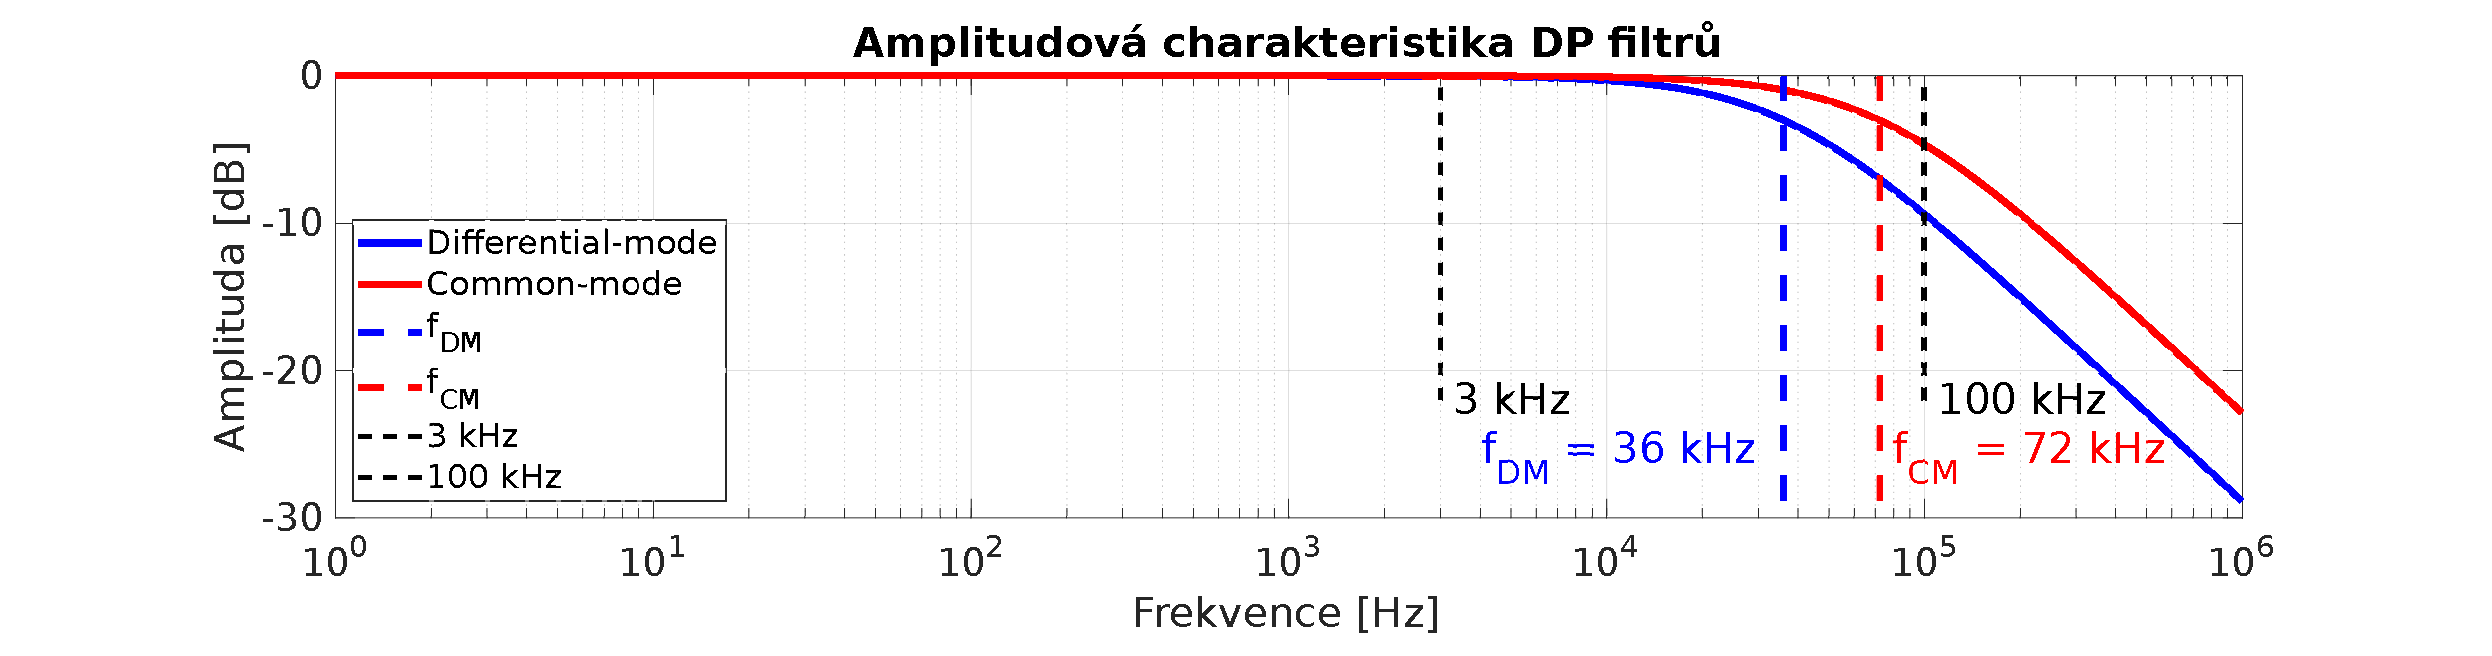
\includegraphics[width=0.9\textwidth]{kapitola2/figures/filter_f_char.eps}
	\caption{Útlumové charakteristiky pro dolnopropustné filtry prvního řádu \textit{CM} a \textit{DM} připojené mezi diferenciální zesilovač \textit{INA241B1} a snímací odpor}
	\label{fig::LP_filtter}
\end{figure}


Frekvence užitečného signálu by měla být menší než  \(\frac{1}{10}\) nejnižší mezní frekvence z obou filtrů.
To je jeden z důvodů, proč je v řešení \nameref{section::dds_implementation} maximální nastavitelná frekvence výstupního proudu stanovena na \SI{3}{\kilo\hertz}, 
vyznačená v amplitudové charakteristice na \oref{fig::LP_filtter}.
Maximální reálná frekvence bude ovlivněna indukčností zátěže.

\section{CAN Bus Driver}
\label{section::CAN_Bus_Driver}

Při vedení vodivých cest pro \textit{CAN bus} byly využity diferenciální páry s řízenou diferenciální impedancí o velikosti \SI{120}{\ohm}. 
Každá deska má dva možné způsoby připojení ke sběrnici \textit{CAN}. 
První je přes \textit{\textit{THT} pass throug header}, 
kde se desky skládáním do sebe automaticky připojí k \textit{CAN} sběrnici, viz zelený rámeček v \oref{fig::CAN_connector}. 
Druhou možností jsou dva konektory, kde jeden slouží jako vstup a druhý jako výstup \textit{CAN} sběrnice, viz bílý rámeček v \oref{fig::CAN_connector}. 
Vzhledem k tomu, že sběrnice vzniká skládáním desek, je důležité vyřešit její terminaci.


\begin{figure}[htpb]
	\centering
	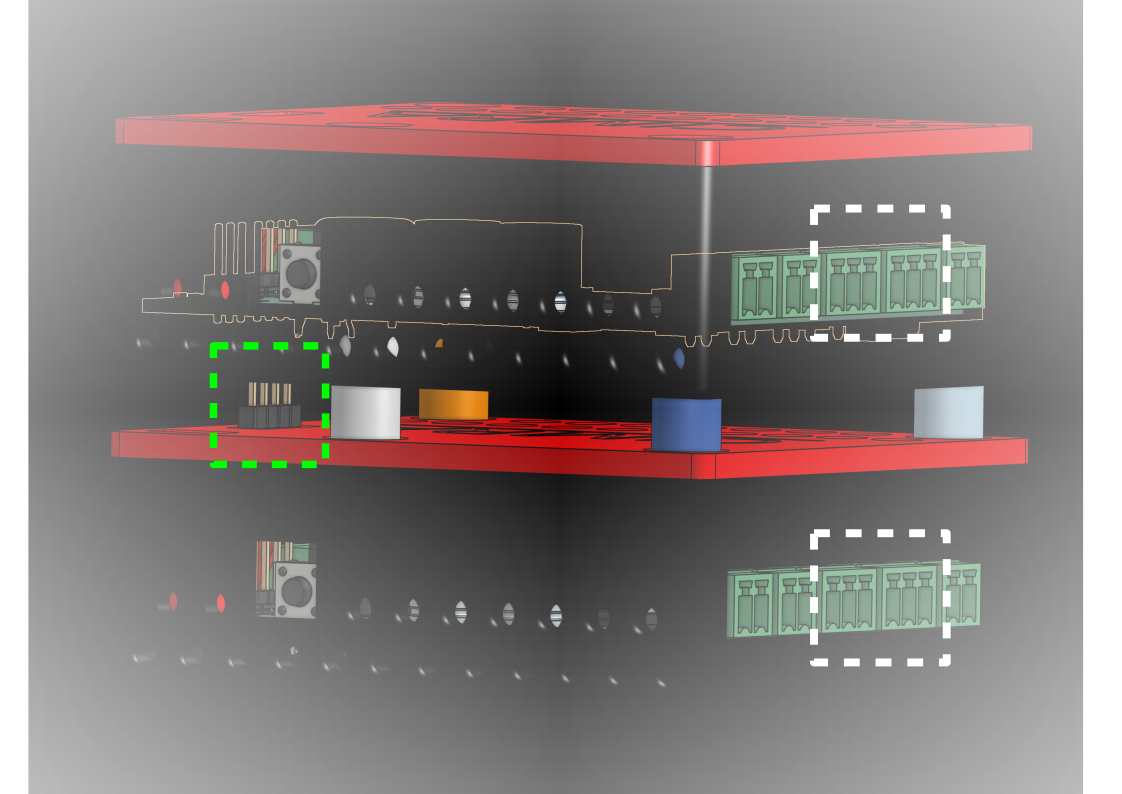
\includegraphics[width=0.9\textwidth]{kapitola2/figures/can_connector.png}
	\caption{Možnosti připojení ke \textit{CAN} sběrnici, \textbf{zelený} rámeček \textit{\textit{THT} pass throug header}, přes konektory v  \textbf{bílém} rámečku}
	\label{fig::CAN_connector}
\end{figure}	


Na desce nejsou přítomny žádné terminační odpory, a to z toho důvodu, že terminační odpory by měly být přítomny pouze na začátku a 
konci sběrnice.
Vzhledem ke konstrukci, kdy sběrnice vzniká skládáním desek, 
by terminační odpor měla obsahovat pouze první a poslední deska na sběrnici. 
Aby mohly být všechny desky plošných spojů stejné, tj. bez vytváření dedikovaných terminačních desek \textit{MoSeZ}, 
respektive desek, které mají terminační odpory připájené, bylo rozhodnuto, že terminační odpory se budou na první a 
poslední desku připojovat do jednoho z \textit{CAN} konektorů, viz bílý rámeček v \oref{fig::CAN_connector}.


\section{Interface}

Každý ze vstupů je chráněn \textit{TVS} diodami proti přepětím, 
zejména proti \textit{ESD}.
Pro zajištění dobré funkce \textit{TVS} diod je nutné je umístit co nejblíže ke konektorům a headerům.
V nové revizi je možnost měřit až dva analogové signály s rozsahem \SIrange{0}{2,5}{\volt} připojené k desce.
Hlavním záměrem je možnost zavedení informace o stavu aktuátorů do zpětné vazby regulátoru.
Toho se v této práci využívá při sledování polohy jádra voicecoilu pomocí vhodně umístěného hallova senzoru, viz \nameref{sec::voicecoil_function}.
Ovšem lze tyto vstupy využít pro měření libovolného analogového napětí v rozsahu \SI{3,3}{\volt}.

Ze staré revize zůstávají dva napájecí dvoupinové konektory, dva \textit{CAN} třípinové konektory, 
jeden dvoupinový konektor pro proudový výstup, 
třípinový header pro komunikaci přes \textit{UART} a jeden čtyřpinový header pro rozvod \textit{CAN} a napětí \SI{3,3}{\volt}.

\begin{figure}[htpb]
    \centering
    \includegraphics[width=0.9\textwidth]{kapitola1/figures/pcb_fornt.jpg}
    \caption{Přední strana DPS MoSeZ rev. B, zadní strana DPS viz příloha A: \nameref{priloha:pcb_back}}
    \label{fig::mosez_pcb_front}
\end{figure}

